% -*- TeX-master: "all_the_notes.tex" -*-


\section{RF    SQUID     (Flux    qubit).     $     E_J/E_C\sim    50
  $ \label{sec:rfSquid}}

\begin{framed}\noindent
  \noindent  The RF  SQUID composes  of a  JJ in  a loop  with a  big
  inductor.   \red{This inductor  was neglected  for the  CPB in  the
    previous section, since $E_C,E_J>>E_L$}.
  \begin{center}
    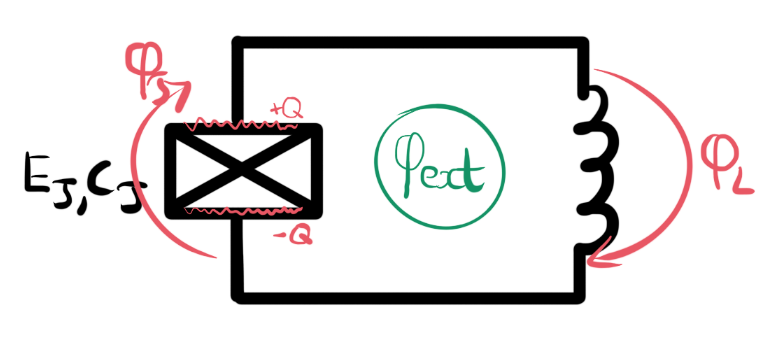
\includegraphics[height=4.5cm]{flux_1}
  \end{center}
\end{framed}


\subsection{Regimes of RF SQUIDs \cite{orlando1999}}
\label{sec:regimes-rf-squids}

Taking  the  loop inductance  $L_s$  and  the  inductance of  the  JJ
$L_J=\frac{\Phi_{0}}{2\pi  I_0}$ (see  \autoref{eq:jj-inductance}) we
have regimes when

\begin{itemize}
\item $L_J >> L_S$ - the current  induced in the loop (by the biasing
  flux) is negligible compared to the current on the JJ:
  \begin{itemize}
  \item \textbf{Aluminium loops};
  \item $E_C = \frac{e^2}{2C}$
  \item $E_J = \frac{I_0\Phi_0}{2\pi}$
  \item Negligible inductance energy of the loop (loop except the JJ)
  \item Use number is a good quantum number
  \end{itemize}
\item $L_J << L_S$ - the current  induced in the loop (by the biasing
  flux) is important:
  \begin{itemize}
  \item \textbf{Niobium};
  \item The quantum variables can be related to the flux in the loops
    and their time derivatives;
  \item Circulating current states - persistent current states.
  \end{itemize}
\end{itemize}

The paper then goes onto  the standard derivation of Hamiltonian from
the Lagrangian  - applying the tight  binding model for two  parts of
the wavefunction in the different minima at different biasing fields.

\subsection{Hamiltonian}
\label{sec:hamiltonian}

\begin{enumerate}
\item \red{\textbf{Potential energy part}} comes  from the JJ and the
  inductor, where we use the phase quantisation in a loop to get

  {\begin{equation}
      \label{l3-energy1}
      \begin{aligned}
        U          =           1          -E_J\cos(\phi_J)          +
        \frac{\Phi_0^2}{(2\pi)^22L}(\phi_\text{ext}-\phi_J)^2,
      \end{aligned}
    \end{equation}}
  \begin{figure}[h]
    \centering 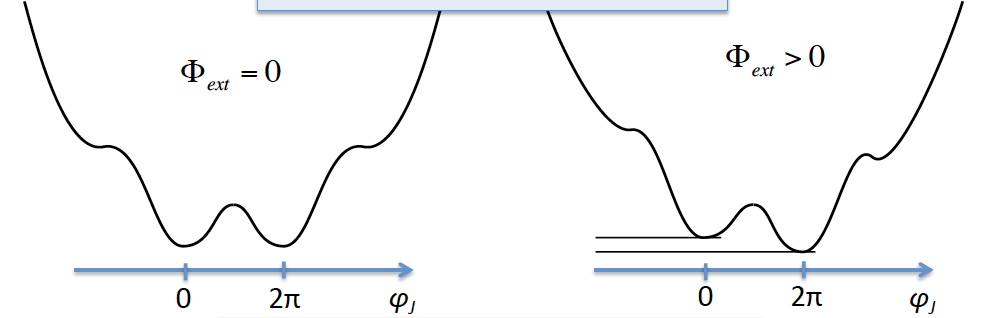
\includegraphics[height=4cm]{phij}
  \end{figure}

  \noindent
  \noindent resulting in a `wiggled' parabollic potential.

\item \red{\textbf{The  charging kinetic  part}} is from  the voltage
  being induced by the changing flux on the JJ

  \begin{equation}
    T = \frac{C_J}{2}\dot{\Phi}_J^2.
  \end{equation}

\item The full \red{\textbf{Lagrangian}} now reads
  \begin{equation}
    \mathcal{L} = T - U = \frac{C_J}{2}\dot{\Phi}_J^2 + E_J\cos(\phi_J) - \frac{\Phi_0^2}{(2\pi)^22L}(\phi_\text{ext}-\phi_J)^2.
  \end{equation}

\item The \textbf{\red{conjugate momentum}}
  \begin{equation}
    Q_J = \frac{d\mathcal{L}}{d\dot{\Phi}_J} = C_J\dot{\Phi}_J,
  \end{equation}
  \noindent is just an offset of  the induced charge on the capacitor
  due to the JJ voltage.

\item So we arrive at the following set of operators

  \begin{equation}
    { \textcolor{blue}{\mathbf{x\leftrightarrow \Phi \leftrightarrow \phi} \text{ (position/flux) }}\qquad \textcolor{red}{\mathbf{p\leftrightarrow Q \leftrightarrow N \text{ (momentum/electrons) }}}}
  \end{equation}

  \noindent with the commutation relations:

  \begin{align}
    \left[\blue{x},\red{p}\right] & =i\hbar & \left[\blue{\Phi},\red{Q}\right] & = i\hbar & \left[\phi,N\right] & = \frac{2\pi}{\frac{h}{2e}}\left[\Phi,Q\right]\frac{1}{2e} = i\\
    \red{\hat{p}} & = -i\hbar\ipartial{}{\blue{x}} & \hat{\red{Q}} & =-i\hbar\ipartial{}{\blue{\Phi}} & \hat{\red{N}} & =-i\ipartial{}{\blue{\phi}}
  \end{align}

\item\

\begin{framed}\noindent
  Expressing the \red{\textbf{Hamiltonian}} in the standard fashion

  \begin{equation}
    \begin{aligned}
      \mathcal{H} & = \hat{Q}_J\dot{\hat{\Phi}}_J - \mathcal{L}\\
      & = \frac{\hat{Q}_J^2}{2C_J} - E_J\cos(\hat{\phi}_J) + \frac{\Phi_0^2}{(2\pi)^22L}(\phi_\text{ext}-\hat{\phi}_J)^2\\
      &   =   \mathbf{\red{E_C{\hat{N}^2}-  E_J\cos(\hat{\phi}_J)   +
          E_L(\phi_\text{ext}-\hat{\phi}_J)^2}}\qquad      E_c      =
      \frac{(2e)^2}{2C_J}\quad E_L = \frac{\Phi_0^2}{(2\pi)^22L}.
    \end{aligned}
  \end{equation}
\end{framed}

\item\red{\large So  now one  has a parabolic  potential term  in the
    Hamiltonian, unlike in  the Cooper Pair box case  where there was
    only the cosine potential}
  \begin{itemize}
  \item $ \phi_{\text{ext}} $ controls the shape of the potential and
    hence the energies of each eigenstate
  \item $ \phi_{\text{JJ}} $ is the dynamic parameter of the qubit.
  \end{itemize}
\end{enumerate}

\newpage
\subsection{Numerical                   solution                   of
  Hamiltonian\label{subsec:flux_numerical}}
There is  a numerical method  to solve  for the RF-SQUID,  whereby we
dice up the state of the system into individual values at discretised
positions, with as step of $ \Delta \delta $

\[
  \psi \rightarrow \begin{pmatrix}
    \psi(0)\\
    \psi(\Delta \delta)\\
    \psi(2\Delta \delta)\\\vdots
    \\
    \psi(n\Delta \delta)
  \end{pmatrix}
  \equiv
  \begin{pmatrix}
    w_0\\
    w_1\\
    w_2\\
    \vdots\\
    w_{n}
  \end{pmatrix}
\]

\noindent and solve

\begin{equation}\label{eqn:flux_1}
  \begin{aligned}
    \mathcal{H}     \psi    &     =    \left[\red{E_c\hat{N}^2}     -
      \blue{E_J\cos(\hat{\phi}_J) +
        E_L(\phi_\text{ext}-\hat{\phi}_J)^2} \right]\psi\\
    &    =     \left[\red{-E_C\frac{\partial}{\partial\phi_J^2}}    +
      \blue{U(\phi_J)}\right]\psi &\equiv E\psi
  \end{aligned}
\end{equation}

\noindent  for  this   wavefunction  made  up  of  a   lot  of  small
contributions.

\begin{figure}[h]
  \centering 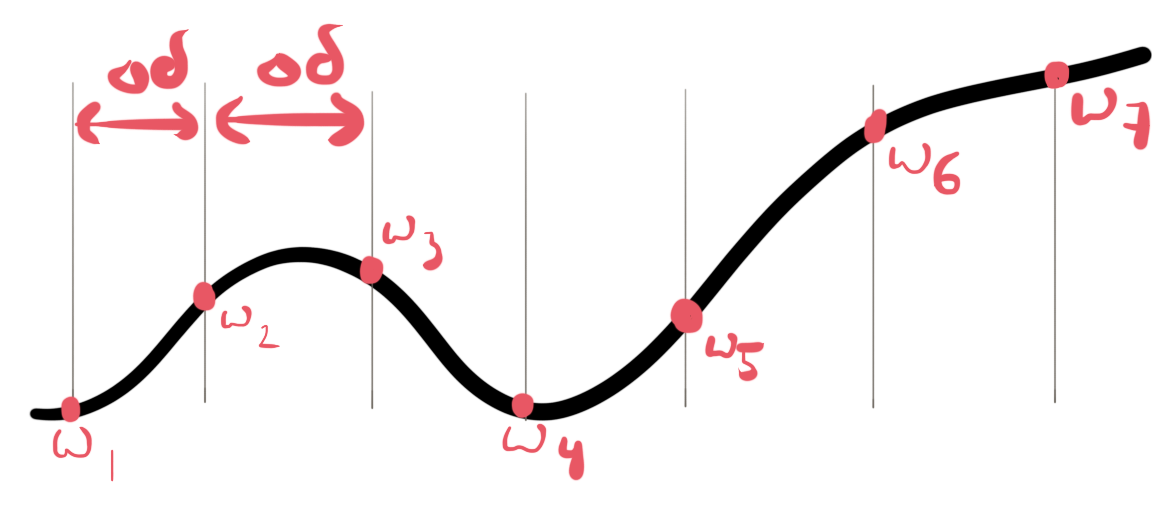
\includegraphics[height=4cm]{dicedUp}
\end{figure}

\noindent

\noindent The derivative, can be evaluated using neighbouring points:

   \begin{equation}\label{eqn:flux_2}
     \frac{d}{d\phi_J^2}\left(\omega_i\right) = \frac{\frac{\omega_{i+1} - \omega_i}{\Delta\delta} - \frac{\omega_{i} - \omega_{i-1}}{\Delta\delta}}{\Delta\delta} = \red{\frac{1}{\Delta\delta^2}\left[\omega_{i+1}+\omega_{i-1}-2\omega_{i}\right]}.
   \end{equation}

   \noindent  We rewrite  Eq.~\eqref{eqn:flux_1} with  the derivative
   Eq.~\eqref{eqn:flux_2} to get
   \begin{equation}
     \begin{aligned}
       & \left[-\frac{E_C}{\Delta\delta^2}\left[\omega_{2}+\omega_{0}-2\omega_{1}\right] + U(w_1)\right]\omega_1 = Ew_1\\
       & \left[-\frac{E_C}{\Delta\delta^2}\left[\omega_{3}+\omega_{1}-2\omega_{2}\right] + U(\omega_2)\right]\omega_2 = Ew_2\\
       & \cdots
     \end{aligned}
   \end{equation}
   \begin{framed}\noindent

     \begin{equation}
       \begin{pmatrix}
         2\frac{E_c}{\Delta\delta^2} + U(w_1) & -\frac{E_c}{\Delta\delta^2} & 0 & 0 \\
         -\frac{E_c}{\Delta\delta^2} & 2\frac{E_c}{\Delta\delta^2} + U(w_2) &   -\frac{E_c}{\Delta\delta^2} & 0\\
         0 & -\frac{E_c}{\Delta\delta^2} & 2\frac{E_c}{\Delta\delta^2} + U(w_3) &   -\frac{E_c}{\Delta\delta^2}\\
         \vdots & \vdots & \vdots & \ddots
       \end{pmatrix}
       \begin{pmatrix}
         w_1\\w_2\\w_3\\\vdots
       \end{pmatrix}
       = E \begin{pmatrix}
         w_1\\w_2\\w_3\\\vdots
       \end{pmatrix}
     \end{equation}

     \noindent where

   \begin{equation}
     \left[
       \begin{aligned}
         \mathbf{U(\phi_J)} & = \mathbf{E_L(\phi_\text{ext} - \phi_J)^2 - E_J\cos(\phi_J)}\\
         E_c & = \frac{(2e)^2}{2C}\\
         E_L & = \frac{\Phi_0^2}{2L(2\pi)^2}\\
         E_J        &        =        \frac{\Phi_0I_c}{2\pi}        =
         \frac{\Phi_0}{2\pi}\frac{\pi\Delta(0)}{2eR}
       \end{aligned}
     \right.
   \end{equation}
 \end{framed}

 The eigentates can be evaluated in \verb|MatLab|:
 \begin{center}
   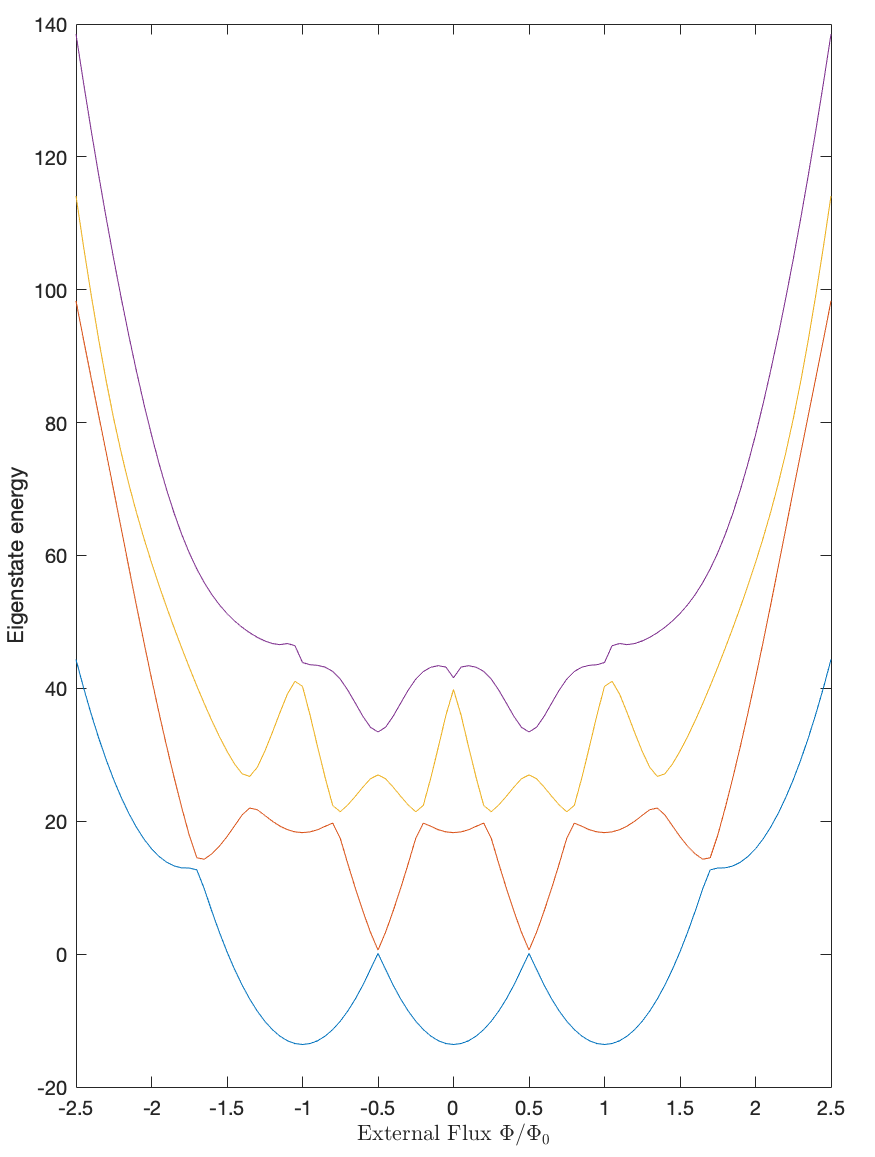
\includegraphics[height=8cm]{flux_simulation_1}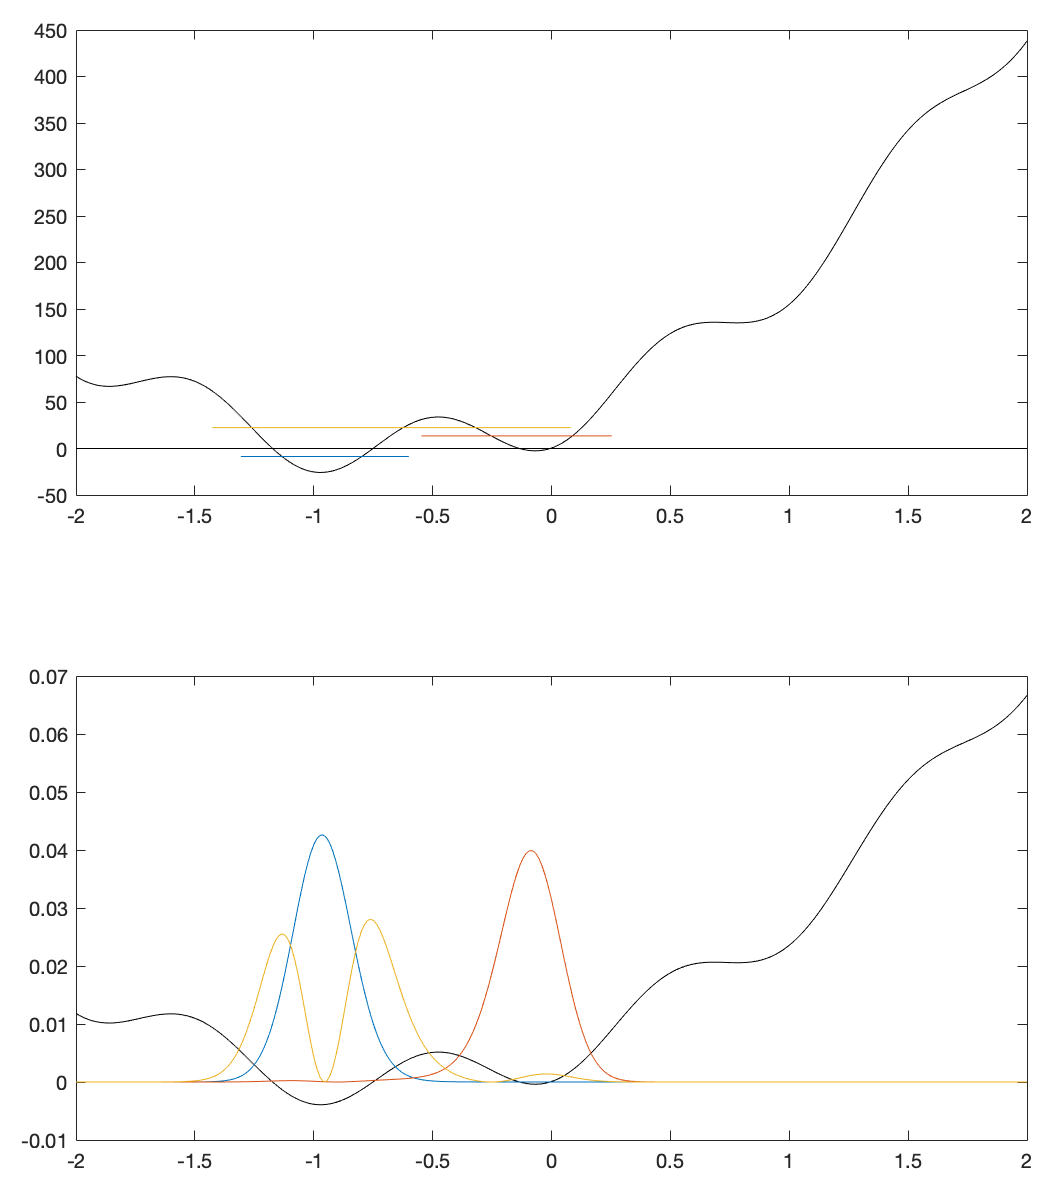
\includegraphics[height=9cm]{flux_simulation_2}
 \end{center}

 \newpage
 \subsection{Solution in the degenerate case}
 There  is a  nice  solution when  eigenstates  are degenerate,  that
 occurs  with  a  symmetrical  double  well  potential.   Eigenstates
 \iket{\psi(0)}   and  \iket{\psi(2\pi)}   constitute   to  the   two
 circulating current directions.

\begin{figure}[h]
  \centering 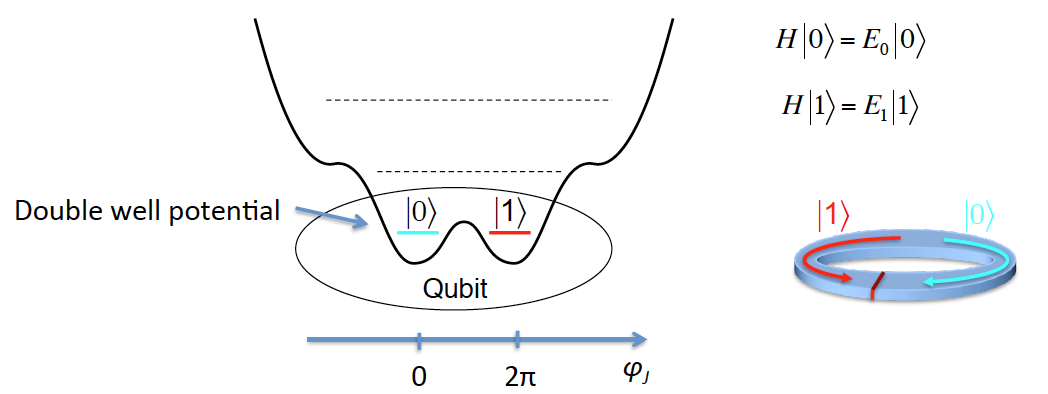
\includegraphics[height=3cm]{double}
\end{figure}

\noindent

\begin{enumerate}
\item We look for contribution to the  wavefunction at $ \phi_J = 0 $
  and  $ \phi_J  =  2\pi $,  `sampling' much  more  strictly than  in
  Section~\ref{subsec:flux_numerical}:
  \[
    \psi \rightarrow \begin{pmatrix}
      \psi(0)\\
      \vdots
      \\
      \psi(n\Delta \delta)
    \end{pmatrix}
    \iratext{$ \Delta = 2\pi, n = 1 $}
    \begin{pmatrix}
      \psi(0)\\
      \psi(2\pi)
    \end{pmatrix} \grey{= \psi(0)\iket{0} + \psi(2\pi)\iket{1}}
  \]

  \noindent looking for solutions to solve

  % \begin{equation}\label{}
  %   \begin{aligned}
  %     \mathcal{H}\psi & = \left[\red{E_с\hat{N}^2} -
  %       \blue{E_J\cos(\hat{\phi}_J) +
  %       E_L(\phi_\text{ext}-\hat{\phi}_J)^2}\right]\psi\\
  %     & = \left[\red{-E_C\frac{\partial}{\partial\phi_J^2}} +
  %       \blue{U(\hat{\phi}_J)}\right]\psi &&\equiv E\psi
  %   \end{aligned}
  % \end{equation}

\item The potential consists of

  \begin{equation}
    \begin{aligned}
      \blue{-E_J\cos(\phi_J)} & \rightarrow \text{ symmetric about } \phi_J = \pi(2n+1)\quad n\in\mathbb{Z}\\
      \blue{E_L(\phi_\text{ext}-\phi_J)^2} & \rightarrow \text{ symmetric about } \phi_J = \phi_\text{ext}.\\
    \end{aligned}
  \end{equation}

\item \blue{\noindent  Thus the  potential is symmetrical  and states
    \iket{0} or \iket{1} are degenerate if

  \[
    \phi_\text{ext}\approx\pi+\delta\phi.
  \]}

\begin{figure}[h]
  \begin{center}
    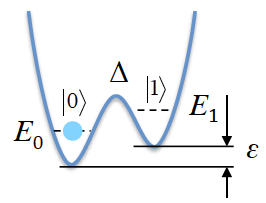
\includegraphics[height=3cm]{l3degen}
    \caption{\small The two  lowest energies for the  system near the
      double  potential  well.    The  loop  is  biased   by  a  flux
      corresponding  to  $\phi_\text{ext}\approx\pi$  - half  a  flux
      quantum.\label{fig:l3degen}}
  \end{center}
\end{figure}

\item  The  energy  difference  between  the  two  wells  located  at
  $\phi_{J1}=0$  and  $  \phi_{J2}=2\pi   $  (or  equivalently  at  a
  separation of 2$ \pi $).

  \begin{equation}
    \begin{aligned}
      \varepsilon &= E_0 - E_{2\pi} \\
      & = \left[-E_J\cos(0) + E_L(\phi_\text{ext}-0)^2\right] - \left[-E_J\cos(2\pi) + E_L(\phi_\text{ext}-2\pi)^2\right]\\
      & = E_L\bigg[\phi_\text{ext}^2 -\phi_\text{ext}^2 +4\pi\phi_\text{ext} -4\pi^2\bigg] =  4\pi E_L\bigg[\phi_\text{ext} -\pi\bigg]\\
      & \approx 4\pi E_L\bigg[\pi+\delta\phi -\pi\bigg] = 4\pi E_L\delta\phi = 4\pi \frac{\Phi_0^2}{(2\pi)^22L} \delta\phi = {\frac{1}{2\pi}\frac{\Phi_0^2}{2L}\delta\phi}\\
      \blue{\varepsilon} & = \blue{\frac{\Phi_0}{2L}\delta\Phi = I_p\delta\Phi}\\
      & \red{\text{Recalling that } E_J = \frac{\Phi_0 I_c}{2\pi}, \text{ where $ I_c $ is the maximal persistent current (critical current)}}\\
    \end{aligned}
  \end{equation}

  \begin{framed}\noindent
  \item  So  for   the  potential  part  accounts   for  two  states,
    \iket{\psi(0)} and  \iket{\psi(2\pi)} at two  different energies,
    which we can write as a diagonal matrix

  \begin{equation}
    \blue{U =
      \kbordermatrix{
        & \iket{\psi(0)} & \iket{\psi(2\pi)}\\
        \bra{\psi(0)} & \frac{\varepsilon}{2} & 0\\
        \bra{\psi(2\pi)} & 0& -\frac{\varepsilon}{2}\\
      } \qquad \qquad \varepsilon = \frac{\Phi_0}{2L}\delta\Phi = I_p\delta\Phi}.
  \end{equation}

\end{framed}

\item               The               \red{kinetic               term
    $ \red{-E_C\frac{\partial}{\partial\phi_J^2}}  $} is  evaluted as
  in Chapter~\ref{subsec:flux_numerical}

  \begin{equation}\label{}
    \begin{aligned}
      \frac{d}{d\phi_J^2}\omega_i & = \frac{\frac{\omega_{i+1} - \omega_i}{\Delta\delta} - \frac{\omega_{i} - \omega_{i-1}}{\Delta\delta}}{\Delta\delta} = \red{\frac{1}{\Delta\delta^2}\left[\omega_{i+1}+\omega_{i-1}-2\omega_{i}\right]}\\
      \bullet \frac{d}{d\phi_J^2}\psi(0) & = \frac{1}{(2\pi)^2}\left[\psi(2\pi) + \grey{\psi(-2\pi)} - 2\psi(0)\right] \grey{\approx} \frac{1}{4\pi^2}\left[\psi(2\pi) - 2\psi(0)\right]\\
      \bullet\frac{d}{d\phi_J^2}\psi(2\pi)             &            =
      \frac{1}{(2\pi)^2}\left[\grey{\psi(4\pi)}    +   {\psi(0)}    -
        2\psi(2\pi)\right]                             \grey{\approx}
      \frac{1}{4\pi^2}\left[\psi(0) - 2\psi(2\pi)\right],
    \end{aligned}
  \end{equation}

  \noindent where  we assume  that for the  lowest energy  states the
  wavefucntion      is     negligible      outside     the      well:
  $ \psi(4\pi) = \psi(-2\pi) = 0 $.

\item In matrix form this looks like

  \begin{equation}
    \red{-E_C\frac{d}{d\phi_J^2} = \kbordermatrix{
        & \iket{\psi(0)} & \iket{\psi(2\pi)}\\
        \bra{\psi(0)} & \frac{1}{4\pi^2}2E_C & -\frac{1}{4\pi^2}E_C\\
        \bra{\psi(2\pi)} & -\frac{1}{4\pi^2}E_C& \frac{1}{4\pi^2}2E\\
      } \equiv \kbordermatrix{
        & \iket{\psi(0)} & \iket{\psi(2\pi)}\\
        \bra{\psi(0)} & 0 & -\frac{\Delta}{2} \\
        \bra{\psi(2\pi)} & -\frac{\Delta}{2}& 0\\
      }\qquad\Delta = \frac{2E_C}{4\pi^2}	}
  \end{equation}

\item\

\begin{framed}\noindent
  The Hamiltonian can be written as that for a two level system

  \begin{equation}
    \begin{aligned}
      \mathcal{H} &\approx -\frac{\varepsilon}{2}\sigma_z - \frac{\Delta}{2}\sigma_x = \kbordermatrix{ &  \iket{\psi(0)} & \iket{\psi(2\pi)}\\
        \bra{\psi(0)}  & -\varepsilon/2  &  -\Delta/2\\ \bra{\psi(2\pi)}  &
        -\Delta/2& \varepsilon/2 }
      \qquad \red{\text{when } \phi_\text{ext} \approx\pi} \\
      \varepsilon & = \frac{\Phi_0}{2L}\delta\Phi  \qquad\qquad \text{controlled by bias flux}\\
      \Delta & = \frac{2E_C}{4\pi^2} \qquad\qquad\text{anticrossing energy
        between states \iket{0} and \iket{1}}
    \end{aligned}
  \end{equation}
\end{framed}

\item Solving  as in  Chapter~\ref{sec:firstLecture} using  a unitary
  rotation
  \begin{equation}
    \label{l1-newH}
    \begin{aligned}
      \mathcal{H} & = {-\frac{\epsilon}{2}\sigma_z-\frac{\Delta}{2}\sigma_x}\\
      & = -\frac{\sqrt{\epsilon^2+\Delta^2}}{2}\left(\frac{\epsilon}{\sqrt{\epsilon^2+\Delta^2}}\sigma_z+\frac{\Delta}{\sqrt{\epsilon^2+\Delta^2}}\sigma_x\right)\\
      & = -\frac{\Delta E}{2}\left(\cos\left(\theta\right)\sigma_z+\sin\left(\theta\right)\sigma_x\right)\\
      \Delta E & = \sqrt{\epsilon^2+\Delta^2}\\
      \tan(\theta) & = \frac{\Delta}{\epsilon}\\
    \end{aligned},
  \end{equation}
  \noindent  with eigenvectors  and  eigenvalues being  a mixture  of
  persistence current states \iket{\circlearrowleft}, \iket{\circlearrowright}.

 \begin{equation}
   E = \pm \frac{\Delta E}{2}, \qquad \ket{0} = \begin{pmatrix}
     \cos(\theta/2) \\ \sin(\theta/2)
   \end{pmatrix},  \qquad \ket{1}  =  \begin{pmatrix} \sin(\theta/2)  \\
     -\cos(\theta/2).
   \end{pmatrix}
 \end{equation}
\item     With    states     \iket{\circlearrowleft}    $     \equiv    +I_p     $    and
  $ \iket{\circlearrowright} \equiv -I_p $ the expectation values of the current:
  \begin{equation}
    \begin{aligned}
      \iaverage{I}_{\iket{0}} & = I_p\cos(\theta/2)^2 - I_p \sin(\theta/2)^2 = I_p\cos(\theta)\\
      \iaverage{I}_{\iket{1}} & = I_p\sin(\theta/2)^2 - I_p \cos(\theta/2)^2 = - I_p\cos(\theta)\\
    \end{aligned}
  \end{equation}
\item  Now  we  perform  a  transformation to  rotate  the  state  by
  $ 2\alpha = \theta $

 \begin{equation}
   \mathbf{U=e^{i\frac{\theta}{2}\sigma_y}} =  \cos(\alpha)\mathbb{I}+i\sin(\alpha)\sigma_y
 \end{equation}

 \noindent to rotate the basis  in this plane. \red{\textbf{Note that
     the  transformation   uses  an   angle  HALF  of   the  required
     turn}}. The  {time independent Hamiltonian} will  be transformed
 and evaluating using the commutation relations Eq.\eqref{uniComm1}

 \begin{equation}
   \begin{aligned}
     \mathcal{H}' & = U\mathcal{H}U^{\dagger} = U \bigg[-\frac{\Delta E}{2}\big(\sigma_z\cos(\theta)+\sigma_x\sin(\theta)\big)\bigg]\bigg[\cos(\theta/2)\mathbb{I}\red{-}i\sin(\theta/2)\sigma_y\bigg]\\
     & = U \bigg[\cos(\theta/2)\mathbb{I}+i\sin(\theta/2)\sigma_y\bigg]\bigg[-\frac{\Delta E}{2}\big(\sigma_z\cos(\theta)+\sigma_x\sin(\theta)\big)\bigg]\\
     & = UU\mathcal{H} =-\frac{\Delta E}{2} \bigg[\cos(\theta)\mathbb{I}+i\sin(\theta)\sigma_y\bigg]\bigg[\big(\sigma_z\cos(\theta)+\sigma_x\sin(\theta)\big)\bigg]\\
     & = -\frac{\Delta E}{2}\bigg[\cos^2(\theta)\sigma_z+\sin(\theta)\cos(\theta)\sigma_x+i\sin(\theta)\cos(\theta)\red{\sigma_y\sigma_z}+i\sin^2(\theta)\red{\sigma_y\sigma_x}\bigg]\\
     & = -\frac{\Delta E}{2}\bigg[\cos^2(\theta)\sigma_z+\sin(\theta)\cos(\theta)\sigma_x+i\sin(\theta)\cos(\theta)\red{i\sigma_x}+i\sin^2(\theta)\red{-i\sigma_z}\bigg]\\
     & = -\frac{\Delta E}{2}\sigma_z,
   \end{aligned}
 \end{equation}

\item\

  \begin{framed}\noindent
    \noindent In the rotated frame we  have a two level system, where
    the biasing flux, and the  anticrossing energies come together to
    create new system eigenstates:

    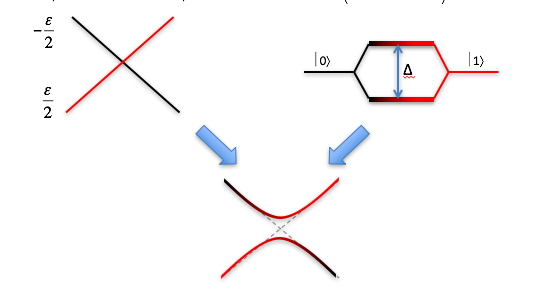
\includegraphics[height=5cm]{together}

    \noindent

  \begin{equation}
    \mathcal{H'} = -\frac{\Delta E}{2}\sigma_z
  \end{equation}

  \red{With  eigenstates  $  \iket{\psi(0)}, \iket{\psi(2\pi)}  $  (mix  of
    persistent current states) at energies
    \begin{equation}
      \pm\frac{\Delta E}{2} \qquad \Delta E = \sqrt{\varepsilon^2 + \Delta^2}\qquad\varepsilon = \frac{\Phi_0}{2L}\delta\Phi  \qquad	\Delta = \frac{2E_C}{4\pi^2}.
    \end{equation}
  }
\end{framed}
\end{enumerate}

\noindent    Fig.\ref{fig:l3wavefun}    depicts   the    approximated
wavefunctions and  Fig.\ref{fig:l3energy} the energies  for different
external fields.

\begin{figure}[h]
  \centering 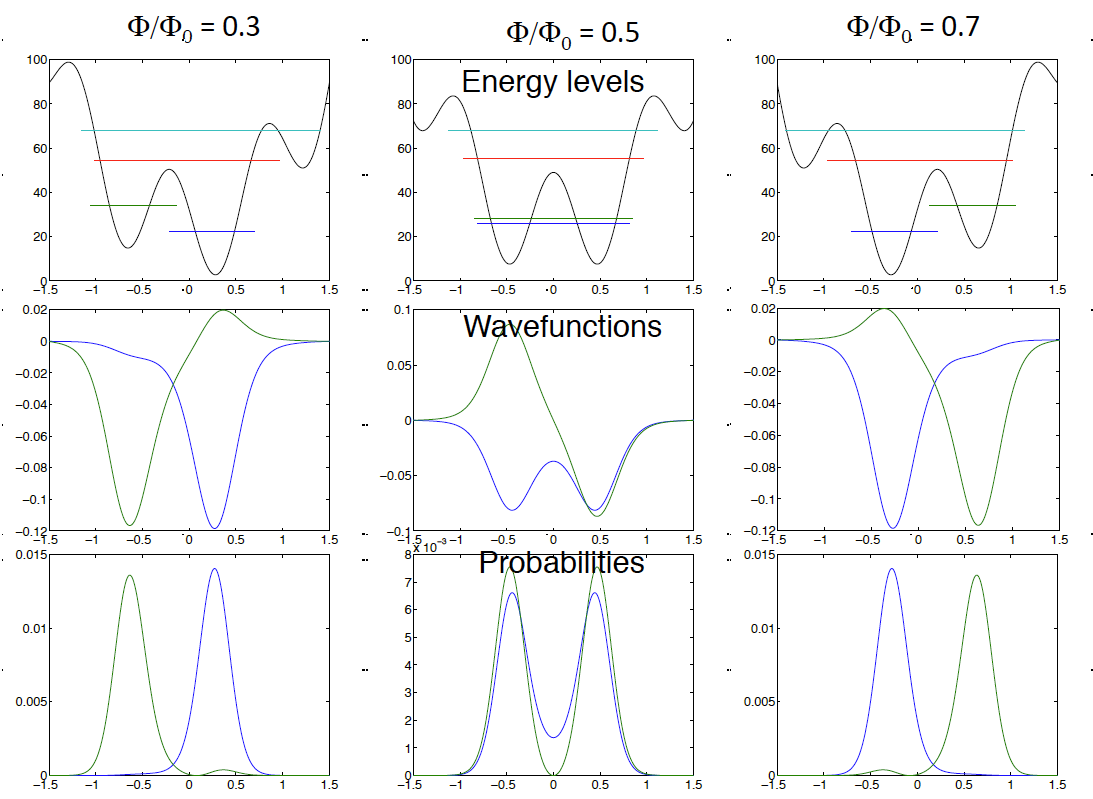
\includegraphics[height=10cm]{l3wavefun}
  \caption{The  wavefunctions  of  the  RF SQUID  as  a  function  of
    $\phi_J$  for different  external flux  $\phi_\text{ext}$ biases.
    Notice how the  different flux biases change the  symmetry of the
    potential and the shape of the wavefunctions}
  \label{fig:l3wavefun}
\end{figure}

\begin{figure}[h]
  \begin{center}
    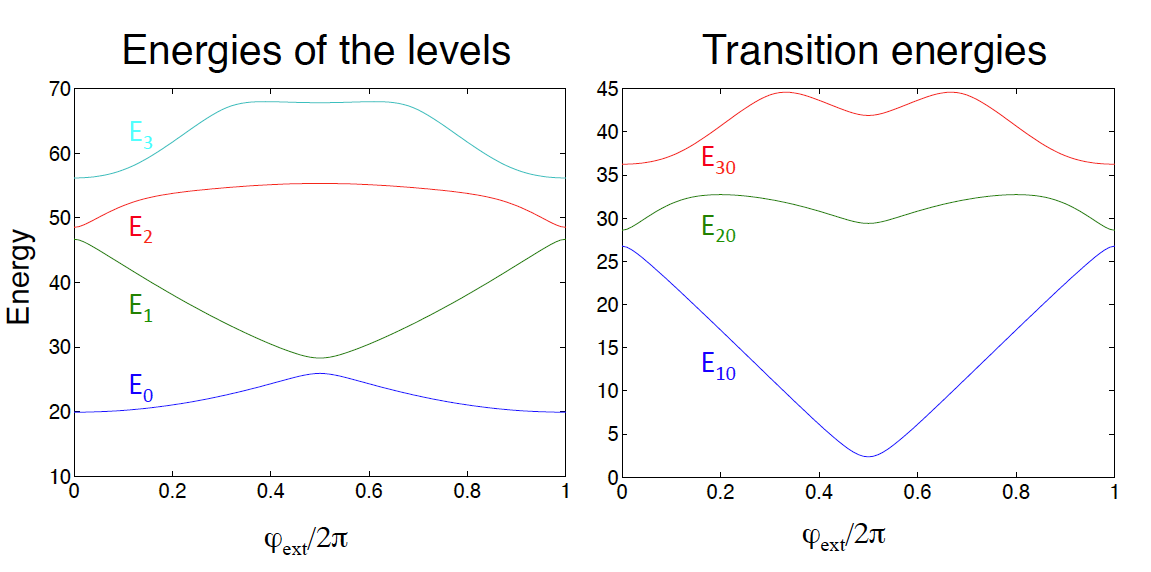
\includegraphics[height=7cm]{l3energy}
    \caption{\small  The energy  levels  and their  differences as  a
      function  of the  \textbf{applied flux}  $\phi_\text{ext}$.  At
      the    degeneracy     point,    the    levels     come    close
      together.\label{fig:l3energy}}
  \end{center}
\end{figure}

\newpage

 \subsection{Question about fabrication}
 There is  a technological  limitation to this  kind of  device. Once
 needs a large inductance $L$, but be able to keep a relatively small
 size. Otherwise the capacitance $ C $ of the system grows too large,
 which prevents the tunnelling of the localised states.

 A proposal  is to replace  the classical  inductor with a  JJ, which
 provides plenty  of inductance,  while keeping a  considerable size.
 Will it work?  Lets evaluate the potential energy

 \begin{equation}
   \left\lbrace\begin{aligned}
       U^{\text{potential}} & = -E_J\cos(\phi_{J1}) - \alpha E_J\cos(\phi_{J2})\\
       \phi_{J1} - \phi_{J2} & = \phi_\text{ext}
     \end{aligned}\right. \Rightarrow
   \begin{aligned}
     &-E_J\cos(\phi_{J1}) - \alpha E_J\cos(\phi_{J1}-\phi_\text{ext})\\
     & = -E_J\bigg[\cos(\phi_{J1}-\frac{\phi_\text{ext}}{2}+\frac{\phi_\text{ext}}{2}) + \alpha\cos(\phi_{J1}-\frac{\phi_\text{ext}}{2}-\frac{\phi_\text{ext}}{2})\bigg]\\
     & = -E_J\bigg[\cos(\phi'+\frac{\phi_\text{ext}}{2}) + \alpha\cos(\phi'-\frac{\phi_\text{ext}}{2})\bigg]\\
     & = -E_J\bigg[\cos(\phi')\cos(\frac{\phi_\text{ext}}{2}) + \alpha\cos(\phi')\cos(\frac{\phi_\text{ext}}{2})\\
     & - \sin(\phi')\sin(\frac{\phi_\text{ext}}{2}) + \alpha\sin(\phi')\sin(\frac{\phi_\text{ext}}{2}) \bigg]\\
     &                                                              \approx
     -E_J(1+\alpha)\bigg[\cos(\phi')\cos(\frac{\phi_\text{ext}}{2})\bigg]
   \end{aligned}
 \end{equation}

 \noindent  There is  no parabolic  dependence, making  the localised
 states unsuitable  - the eigenstates  will tunnel across all  of the
 possible wells  formed by the  cosine potential. \textbf{So  this is
   not possible with just replacing an inductor with a JJ.}

 \newpage
